\documentclass[conference,a4paper]{IEEEtran}

% Escritura mejorada de fórmulas matemáticas
\usepackage{amsmath}

% Inserción de gráficos
\usepackage{graphicx}

% Escritura mejorada de tablas
\usepackage{booktabs}
\usepackage{tabularx}

% Escritura mejorada de citas bibliográficas
\usepackage{cite}

% Para codificación UTF-8 y español
\usepackage[utf8]{inputenc}
\usepackage[spanish]{babel}

% Macros traducidas
\def\contentsname{Índice general}
\def\listfigurename{Índice de figuras}
\def\listtablename{Índice de tablas}
\def\refname{Referencias}
\def\indexname{Índice alfabético}
\def\figurename{Fig.}
\def\tablename{TABLA}
\def\partname{Parte}
\def\appendixname{Apéndice}
\def\abstractname{Resumen}
\def\IEEEkeywordsname{Palabras clave}
\def\IEEEproofname{Demostración}

\begin{document}

\title{Recuperación de la Información: Modelos Booleanos y Vectoriales aplicados al Metajuego de Pokémon}

\author{
  \IEEEauthorblockN{Adrián Muñoz Aradilla}
  \IEEEauthorblockA{
    \textit{Dpto. Ciencias de la Computación e Inteligencia Artificial}\\
    \textit{Universidad de Sevilla}\\
    Sevilla, España\\
    adrmunara@alum.us.es}
  
  \and
  
  \IEEEauthorblockN{Rocío Morato Aguilar}
  \IEEEauthorblockA{
    \textit{Dpto. Ciencias de la Computación e Inteligencia Artificial}\\
    \textit{Universidad de Sevilla}\\
    Sevilla, España\\
    rocmoragu@alum.us.es}
}

\maketitle

% Resumen
\begin{abstract}
  Este documento presenta el diseño, desarrollo y evaluación de dos sistemas de Recuperación de Información aplicados al metajuego competitivo del videojuego Pokémon. El objetivo principal es construir una herramienta que permita a los jugadores buscar Pokémon viables mediante consultas de texto libre y consultas estructuradas lógicas, operando sobre un corpus especializado de textos extraído directamente de la comunidad competitiva Smogon. 
  
  Para abordar este problema, se han desarrollado un modelo Booleano de índice invertido basado en la biblioteca \emph{Whoosh}, y un modelo de Espacio Vectorial ponderado mediante el esquema TF-IDF, empleando NLTK para el preprocesamiento lingüístico y scikit-learn. La evaluación de ambos sistemas, llevada a cabo mediante 20 necesidades de información estructuradas, demuestra el contraste entre la alta precisión de las consultas lógicas del modelo booleano frente a la impecable sensibilidad (100\%) y el ordenamiento por relevancia del modelo vectorial, el cual logra alcanzar un \emph{Mean Average Precision} (MAP) global del 55.02\%. El informe concluye con un análisis crítico que justifica las debilidades prácticas del modelo \emph{Bag of Words}.
\end{abstract}

% Palabras claves
\begin{IEEEkeywords}
  Inteligencia Artificial, Recuperación de Información, Modelo Vectorial, TF-IDF, NLTK, Whoosh, Procesamiento de Lenguaje Natural, Smogon.
\end{IEEEkeywords}

\section{Introducción}

En el ámbito del juego competitivo de la saga Pokémon, la construcción de equipos equilibrados (\emph{teambuilding}) es una disciplina analítica compleja. Esta tarea requiere un conocimiento exhaustivo de múltiples variables de juego: estadísticas base, repertorios de movimientos, habilidades, combinaciones de tipos y los roles específicos que cada criatura desempeña en los combates (murallas defensivas, atacantes rápidos, pivotes, etc.).

Para facilitar este proceso, comunidades especializadas como Smogon University~\cite{b1} publican extensos artículos y análisis estratégicos en formato de texto libre. Estos documentos sirven como guía de referencia para los jugadores que buscan optimizar sus equipos.

Este proyecto surge de la necesidad de estructurar y consultar este gran volumen de información textual. Tradicionalmente, la búsqueda de un Pokémon para cubrir un rol se realiza mediante catálogos rígidos, como la Pokédex oficial, que solo permiten filtrar por estadísticas concretas. Sin embargo, en el juego avanzado, los usuarios necesitan realizar búsquedas sobre conceptos abstractos de estrategia competitiva, como por ejemplo \emph{``fast special attacker fairy resistance''} (atacante especial veloz con resistencia al tipo hada).

Para dar solución a este reto, proponemos la implementación de dos motores complementarios de Recuperación de Información (RI): un sistema Booleano estricto y un sistema basado en el Modelo Vectorial empleando el esquema TF-IDF~\cite{b2}. Ambos motores basan su corpus en 50 documentos obtenidos sistemáticamente por técnicas de \emph{web scraping} de los análisis oficiales de Smogon para la actual novena generación. A lo largo de esta memoria, explicaremos las decisiones de preprocesamiento de Lenguaje Natural adoptadas, los fundamentos teóricos, la metodología de validación empírica utilizando 20 necesidades de información complejas, y una comparativa de los resultados obtenidos por ambos motores.

\section{Preliminares y Fundamentos Teóricos}

El desarrollo de sistemas modernos de Recuperación de Información se basa en técnicas matemáticas y de lingüística computacional que permiten extraer el significado semántico del texto. En esta sección se describen los pilares teóricos de nuestros motores de búsqueda.

\subsection{Procesamiento de Lenguaje Natural (PLN)}

En primer lugar, todo el corpus textual recopilado debe someterse a un preprocesamiento estandarizado. Este proceso incluye la \emph{tokenización} mediante expresiones regulares, la conversión de todo el texto a letras minúsculas, y la eliminación del ruido léxico mediante el filtrado de palabras vacías o \emph{stop-words} (tales como artículos y preposiciones comunes del inglés). Finalmente, se aplica la extracción de raíces léxicas, un proceso conocido como \emph{Stemming}. Para nuestro caso de uso, se ha empleado el algoritmo Porter Stemmer proporcionado por la librería NLTK~\cite{b3}. 

Este preprocesamiento es vital porque cumple una doble función: reducir drásticamente el tamaño del vocabulario y homogeneizar variaciones de palabras (por ejemplo, agrupar ``attack'', ``attacks'' y ``attacker'' bajo una misma raíz semántica).

\subsection{Modelo de Indexación Booleano}

El modelo de recuperación Booleano es un método de búsqueda exacta fundamentado en la teoría de conjuntos y el álgebra de Boole. En este sistema, las consultas no se escriben en texto libre, sino que se formulan de manera restrictiva utilizando agrupaciones por paréntesis y operadores lógicos (\texttt{AND}, \texttt{OR}, \texttt{NOT}). 

Para que la recuperación sea eficiente sin tener que leer todos los documentos en cada búsqueda, el sistema construye previamente un \emph{índice invertido}. Un índice invertido es un diccionario en memoria que relaciona cada palabra del vocabulario con una lista de los documentos que la contienen~\cite{b4}. En este proyecto, el modelo booleano se ha implementado apoyándose en la biblioteca de código abierto de Python llamada \emph{Whoosh}, que facilita nativamente estas operaciones de indexación inversa.

\subsection{Modelo Vectorial y TF-IDF}

En contraste con el filtrado binario estricto del modelo Booleano, el modelo vectorial representa tanto a los documentos como a las consultas del usuario como vectores numéricos. Estos vectores se ubican conceptualmente en un espacio multidimensional que consta de $N$ dimensiones (siendo $N$ el tamaño total del vocabulario del corpus). 

Para evitar el problema de que las palabras muy comunes dominen los resultados de búsqueda, se emplea el conocido esquema de ponderación \textbf{TF-IDF} (\emph{Term Frequency - Inverse Document Frequency})~\cite{b5}.

De acuerdo a la teoría de Recuperación de Información~\cite{b8}, el componente de Frecuencia Documental Inversa (IDF) para un término $t$ en un corpus de $N$ documentos se calcula mediante una ecuación de suavizado logarítmico:
\begin{equation}
\label{eq:idf}
idf_{t} = \log\left(\frac{N}{df_{t}}\right)
\end{equation}
donde el denominador $df_{t}$ equivale a la frecuencia documental observada del término $t$ (en cuántos documentos distintos aparece). Por consiguiente, el peso combinado para un término $t$ dentro de un documento concreto $D$ viene dado por el producto escalar:
\begin{equation}
\label{eq:tfidf}
\text{tf-idf}_{t,D} = \text{tf}_{t,D} \times idf_{t}
\end{equation}

Una vez que el corpus y la consulta del usuario se han representado como vectores normalizados en este espacio multidimensional, la relevancia de un documento respecto a la consulta se calcula evaluando la \textbf{Similitud del Coseno} entre ambos vectores:
\begin{equation}
\label{eq:cosine}
\text{sim}(D, Q) = \frac{\sum_{i=1}^{n} \text{tf-idf}_{t_{i},D} \cdot \text{tf-idf}_{t_{i},Q}}{\sqrt{\sum_{i=1}^{n} \text{tf-idf}_{t_{i},D}^2} \sqrt{\sum_{i=1}^{n} \text{tf-idf}_{t_{i},Q}^2}}
\end{equation}

Esta evaluación geométrica permite al sistema elaborar automáticamente un ranking ordenado de los resultados, priorizando aquellos documentos que comparten una mayor afinidad temática con la consulta.

\subsection{Trabajo Relacionado}

La aplicación de técnicas de Procesamiento del Lenguaje Natural sobre documentación de videojuegos es un campo de estudio emergente. Históricamente, las herramientas de la comunidad Pokémon (como calculadoras de daño o simuladores) se han basado en bases de datos relacionales tradicionales. Estas bases de datos solo permiten realizar búsquedas utilizando filtros estructurados simples (como seleccionar un tipo elemental concreto o establecer un límite numérico para una estadística).

Algunos foros especializados incorporan primitivos motores de búsqueda por texto que se limitan a buscar coincidencias literales de cadenas de caracteres. Al carecer de técnicas como el \emph{stemming} o la ponderación TF-IDF, estos buscadores suelen devolver una cantidad masiva de documentos irrelevantes frente a una simple consulta, dificultando enormemente la experiencia del usuario. Nuestro enfoque, utilizando librerías estandarizadas del sector académico e industrial como \emph{scikit-learn}~\cite{b6} y \emph{NLTK}~\cite{b7}, busca introducir un estándar de búsqueda semántica formal en un entorno recreativo donde predominan soluciones informales.

\section{Metodología e Implementación Técnica}

La construcción de los sistemas propuestos se ha dividido lógicamente en tres fases consecutivas: recopilación de datos, diseño de métricas funcionales de validación, y modelado computacional en Python.

\subsection{Elaboración del Corpus y Colección de Datos}

En primer lugar, se hizo uso de la biblioteca de extracción web \emph{BeautifulSoup} para analizar los documentos HTML y extraer el texto plano de los análisis competitivos oficiales. De esta forma se obtuvo la narrativa descriptiva completa concerniente a 50 criaturas Pokémon distintas. Los textos resultantes se almacenaron localmente en archivos `.txt'. 

Seguidamente, para estructurar los datos extraídos, se empleó la clase \texttt{PlaintextCorpusReader} originaria de la librería NLTK. Esta integración permitió cargar el directorio completo de archivos textuales y unificarlos en un entorno de validación conjunta. A través de este proceso de ingesta, se logró extraer y depurar un vocabulario útil superior a las 3400 raíces léxicas distintas.

Para el proceso de vectorización, se desarrolló un tokenizador personalizado en Python. Su metodología se basa en un diseño secuencial de filtrado lingüístico: cada documento se segmenta en sus componentes atómicos fundamentales mediante un algoritmo estandarizado de división (\emph{word\_tokenize}). Seguidamente, se ejecuta un proceso que descarta todos los elementos no alfabéticos, depurando el corpus de signos de puntuación y números. A continuación, el filtro somete las palabras restantes a una validación negativa frente al diccionario universal de \emph{stop-words} en inglés de NLTK, excluyendo artículos y preposiciones. Finalmente, las palabras supervivientes son canalizadas a través del algoritmo \emph{Porter Stemmer}, el cual extrae la raíz lexema inalterada. Esta secuencia finita de operaciones normalizadoras consolida la reducción del vocabulario final recuperable y prepara los textos para ser procesados por el \texttt{TfidfVectorizer}.

\begin{table*}[t]
  \caption{Muestra representativa de 6 de las 20 Necesidades de Información definidas para evaluar los motores de búsqueda.}
  \label{tab:necesidades}
  \centering
  \begin{tabularx}{\textwidth}{p{0.5cm} p{6cm} p{7cm} c}
    \toprule
    \textbf{ID} & \textbf{Consulta de Texto Libre} & \textbf{Consulta Booleana (Lógica Estricta)} & \textbf{Docs. Relevantes} \\
    \midrule
    Q1 & Swords Dance sweeper priority & "Swords Dance" AND (priority OR "Bullet Punch" OR "Sucker Punch") & 3 \\
    \midrule
    Q4 & Stealth Rock physical wall defensive setter & "Stealth Rock" AND defensive AND ("physical wall" OR tank) & 4 \\
    \midrule
    Q7 & Spore sleep status user & Spore OR "sleep powder" OR "put to sleep" & 2 \\
    \midrule
    Q9 & Magic Bounce hazard control & "Magic Bounce" AND (hazard OR control OR defog) & 1 \\
    \midrule
    Q14 & lead hyper offense fast setup & lead AND "hyper offense" AND fast & 1 \\
    \midrule
    Q18 & Will-O-Wisp burn status cripple physical attackers & "Will-O-Wisp" AND (burn OR status OR cripple) & 2 \\
    \bottomrule
  \end{tabularx}
\end{table*}

\subsection{Diseño de las Necesidades de Información}

Para poder evaluar el rendimiento de los motores de manera científica, era fundamental establecer un conjunto de pruebas, conocido en la literatura como \emph{Ground Truth}. Para ello, se redactó un conjunto de 20 necesidades de información distintas basadas en el conocimiento profundo del metajuego de Pokémon, almacenadas en formato \texttt{CSV}. La TABLA~\ref{tab:necesidades} expone una muestra de las lógicas generadas.

Para cada necesidad de información, se definieron manualmente tres componentes clave:
\begin{enumerate}
\item \textbf{La consulta de texto libre}: Emulando cómo buscaría un usuario corriente utilizando lenguaje natural ordinario (por ejemplo, \emph{``Swords Dance sweeper priority''}).
\item \textbf{La consulta estructurada (booleana)}: El planteamiento lógico estricto requerido para que un motor exacto comprenda la misma consulta, utilizando paréntesis y operadores \texttt{AND/OR} (por ejemplo, \emph{`"Swords Dance" AND priority'}).
\item \textbf{El listado de documentos relevantes}: El juicio humano determinístico que indica exactamente qué documentos del corpus son verdaderamente la respuesta correcta a esa consulta, con el fin de poder medir los aciertos y fallos de las máquinas posteriormente.
\end{enumerate}

\subsection{Implementación Computacional de los Motores}

Con los metadatos de validación preparados, se procedió a programar los dos motores. El sistema Booleano se desarrolló invocando las funciones nativas de indexación de la librería externa \emph{Whoosh}. Se definió un esquema lógico donde se indexaron el título y el contenido completo de cada análisis, permitiendo luego realizar consultas lógicas instantáneas sobre su diccionario.

De manera paralela, el motor Vectorial se programó haciendo uso de \emph{scikit-learn}. Empleando nuestro tokenizador personalizado, la clase \texttt{TfidfVectorizer} calculó matemáticamente una matriz bidimensional global ponderada que relaciona los 50 documentos con los más de 3400 términos extraídos del corpus. En el momento de la consulta, la frase introducida por el usuario se transforma matemáticamente a ese mismo espacio dimensional y se computa iterativamente la similitud del coseno respecto a cada archivo para elaborar el ranking descendente.

\section{Resultados y Evaluación}

La fase de evaluación consistió en someter las 20 consultas a ambos motores de búsqueda. Para medir el éxito, se utilizaron dos de las métricas clásicas más reconocidas en la disciplina de la Recuperación de Información: la \textbf{Precisión} (qué porcentaje de lo devuelto es relevante) y la \textbf{Sensibilidad} o \emph{Recall} (qué porcentaje de los relevantes totales se logró recuperar). 

Dado que el modelo Vectorial devuelve resultados ordenados numéricamente por grado de relevancia, se incorporó una tercera métrica crucial: el \textbf{Mean Average Precision (MAP)}~\cite{b8}, que premia a los sistemas que posicionan los resultados relevantes en los puestos más altos de la lista.

Las métricas globales promediadas sobre el conjunto completo arrojaron los siguientes resultados para el motor Vectorial, ilustrados en la \figurename~\ref{fig:metrics}:
\begin{itemize}
\item \textbf{Mean Average Precision (MAP):} 55.02\%
\item \textbf{Precisión Global Promedio:} 7.00\%
\item \textbf{Sensibilidad Global Promedio:} 100.00\%
\end{itemize}

Asimismo, en la \figurename~\ref{fig:ap} se puede apreciar de forma detallada cómo ha oscilado la métrica del \emph{Average Precision} para cada una de las 20 consultas individualmente, demostrando la variabilidad del rendimiento dependiendo de las palabras clave empleadas.

\begin{figure}[htbp]
  \centering
  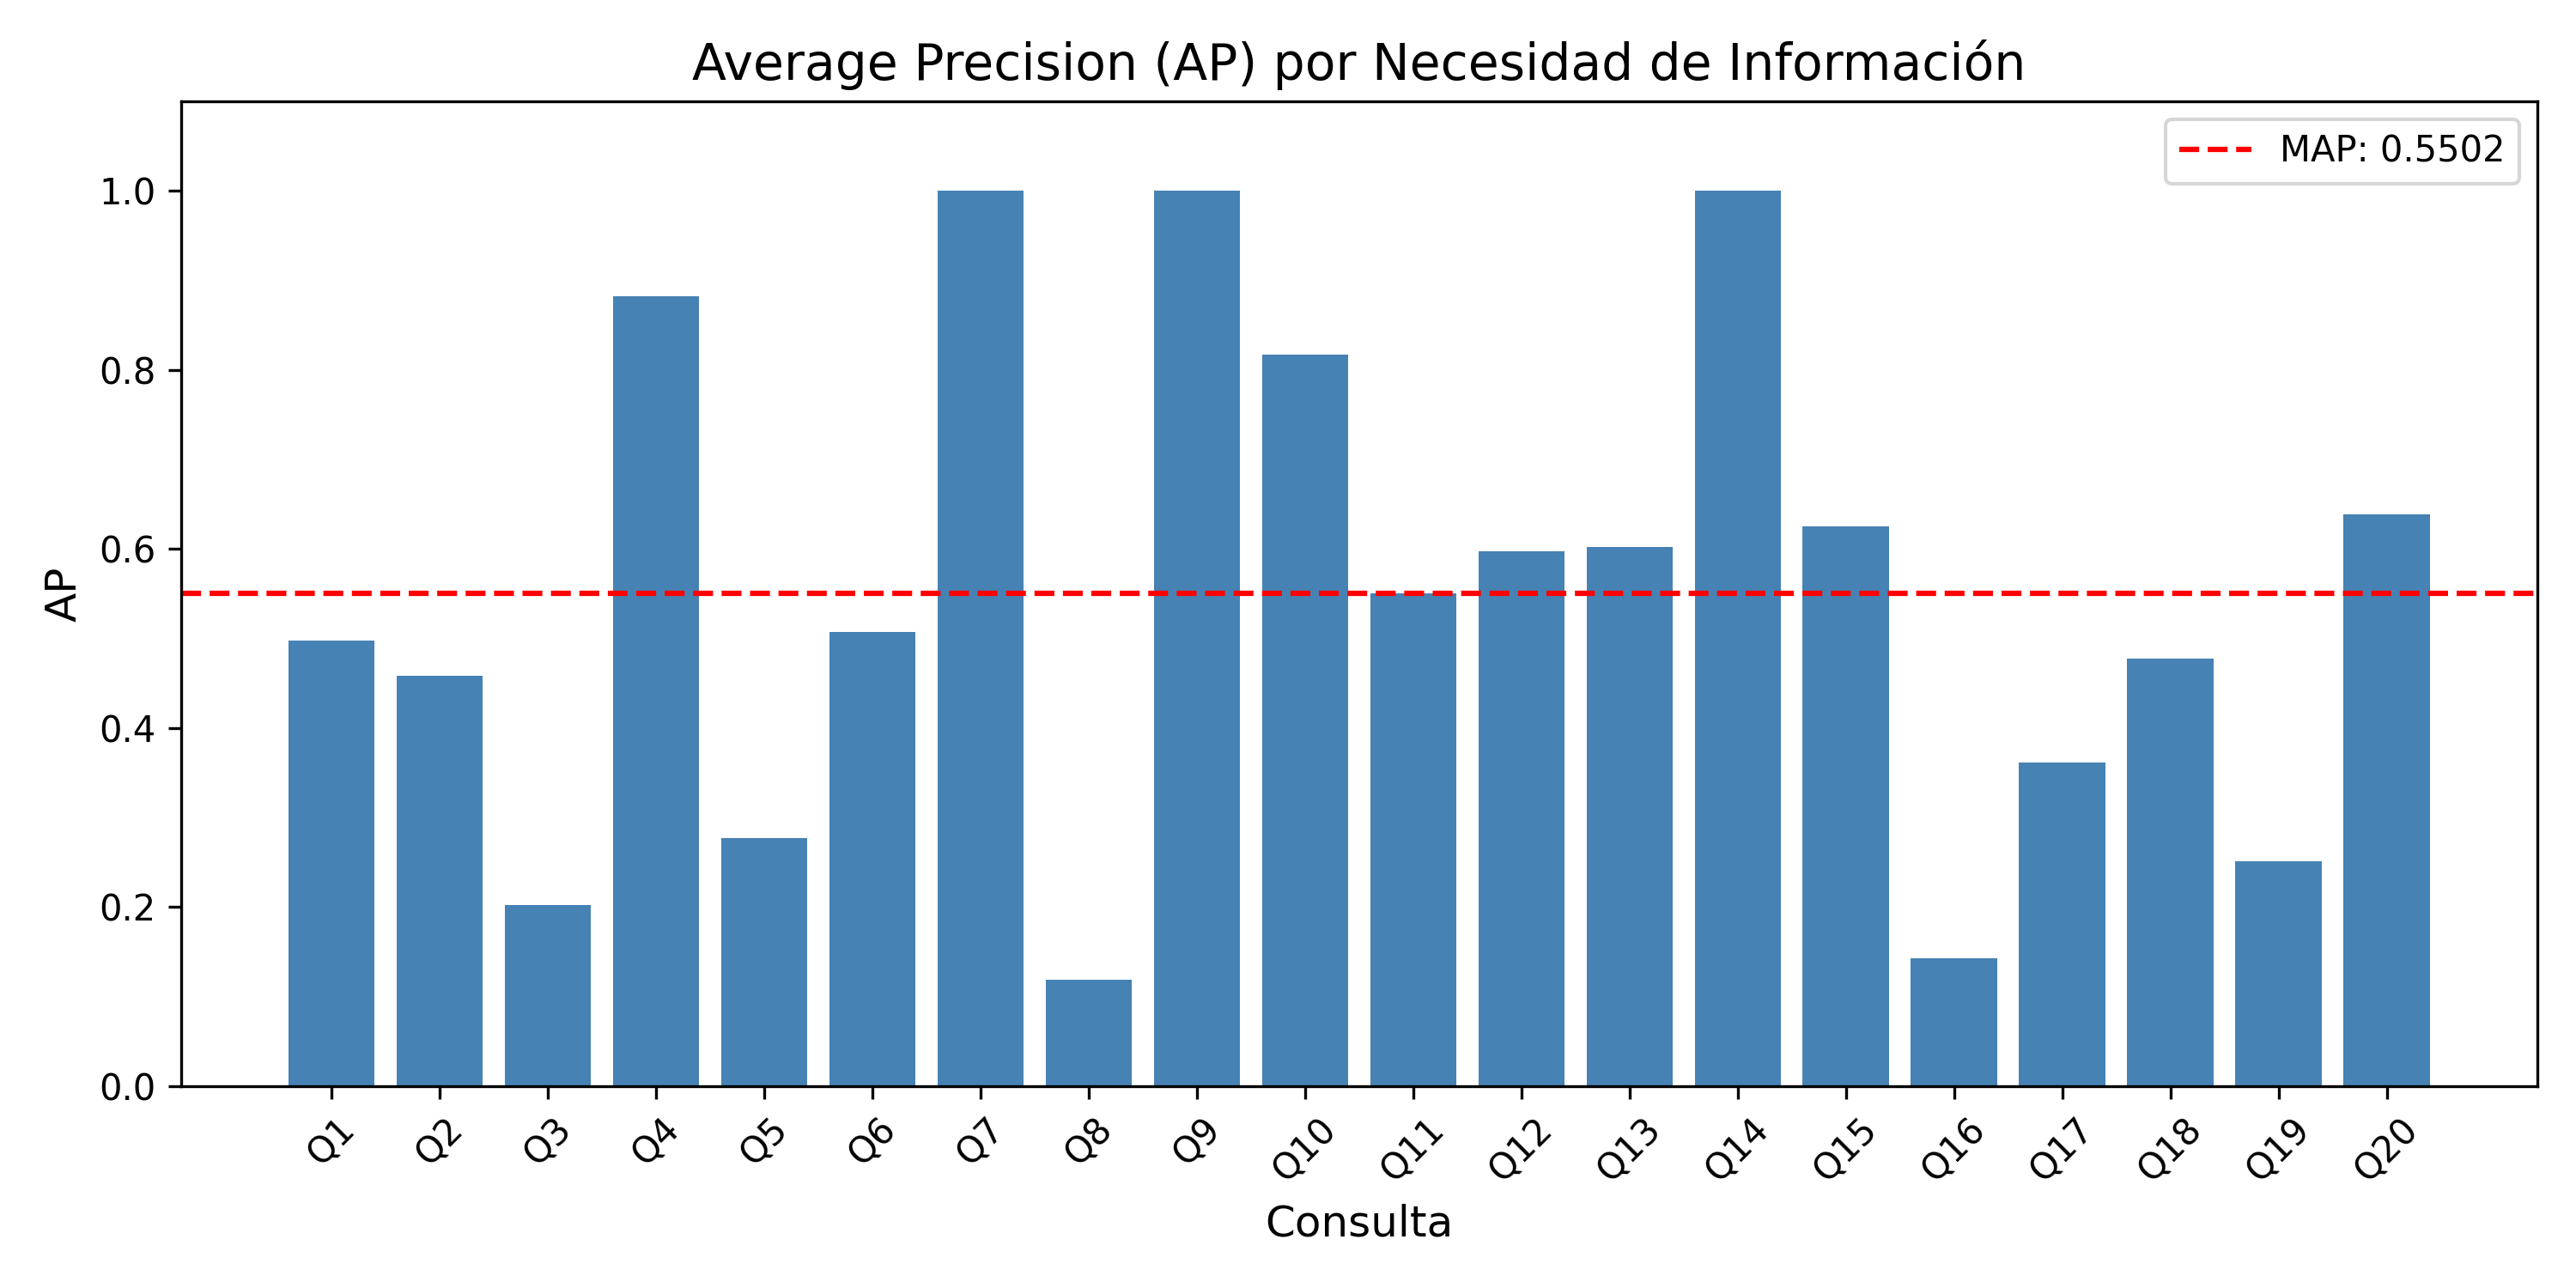
\includegraphics[width=\columnwidth]{ap_chart}
  \caption{Métrica Average Precision (AP) individualizada calculada estadísticamente para el índice Vectorial, desagregada por cada una de las 20 necesidades de información estructuradas (Q1-Q20).}
  \label{fig:ap}
\end{figure}

\begin{figure}[htbp]
  \centering
  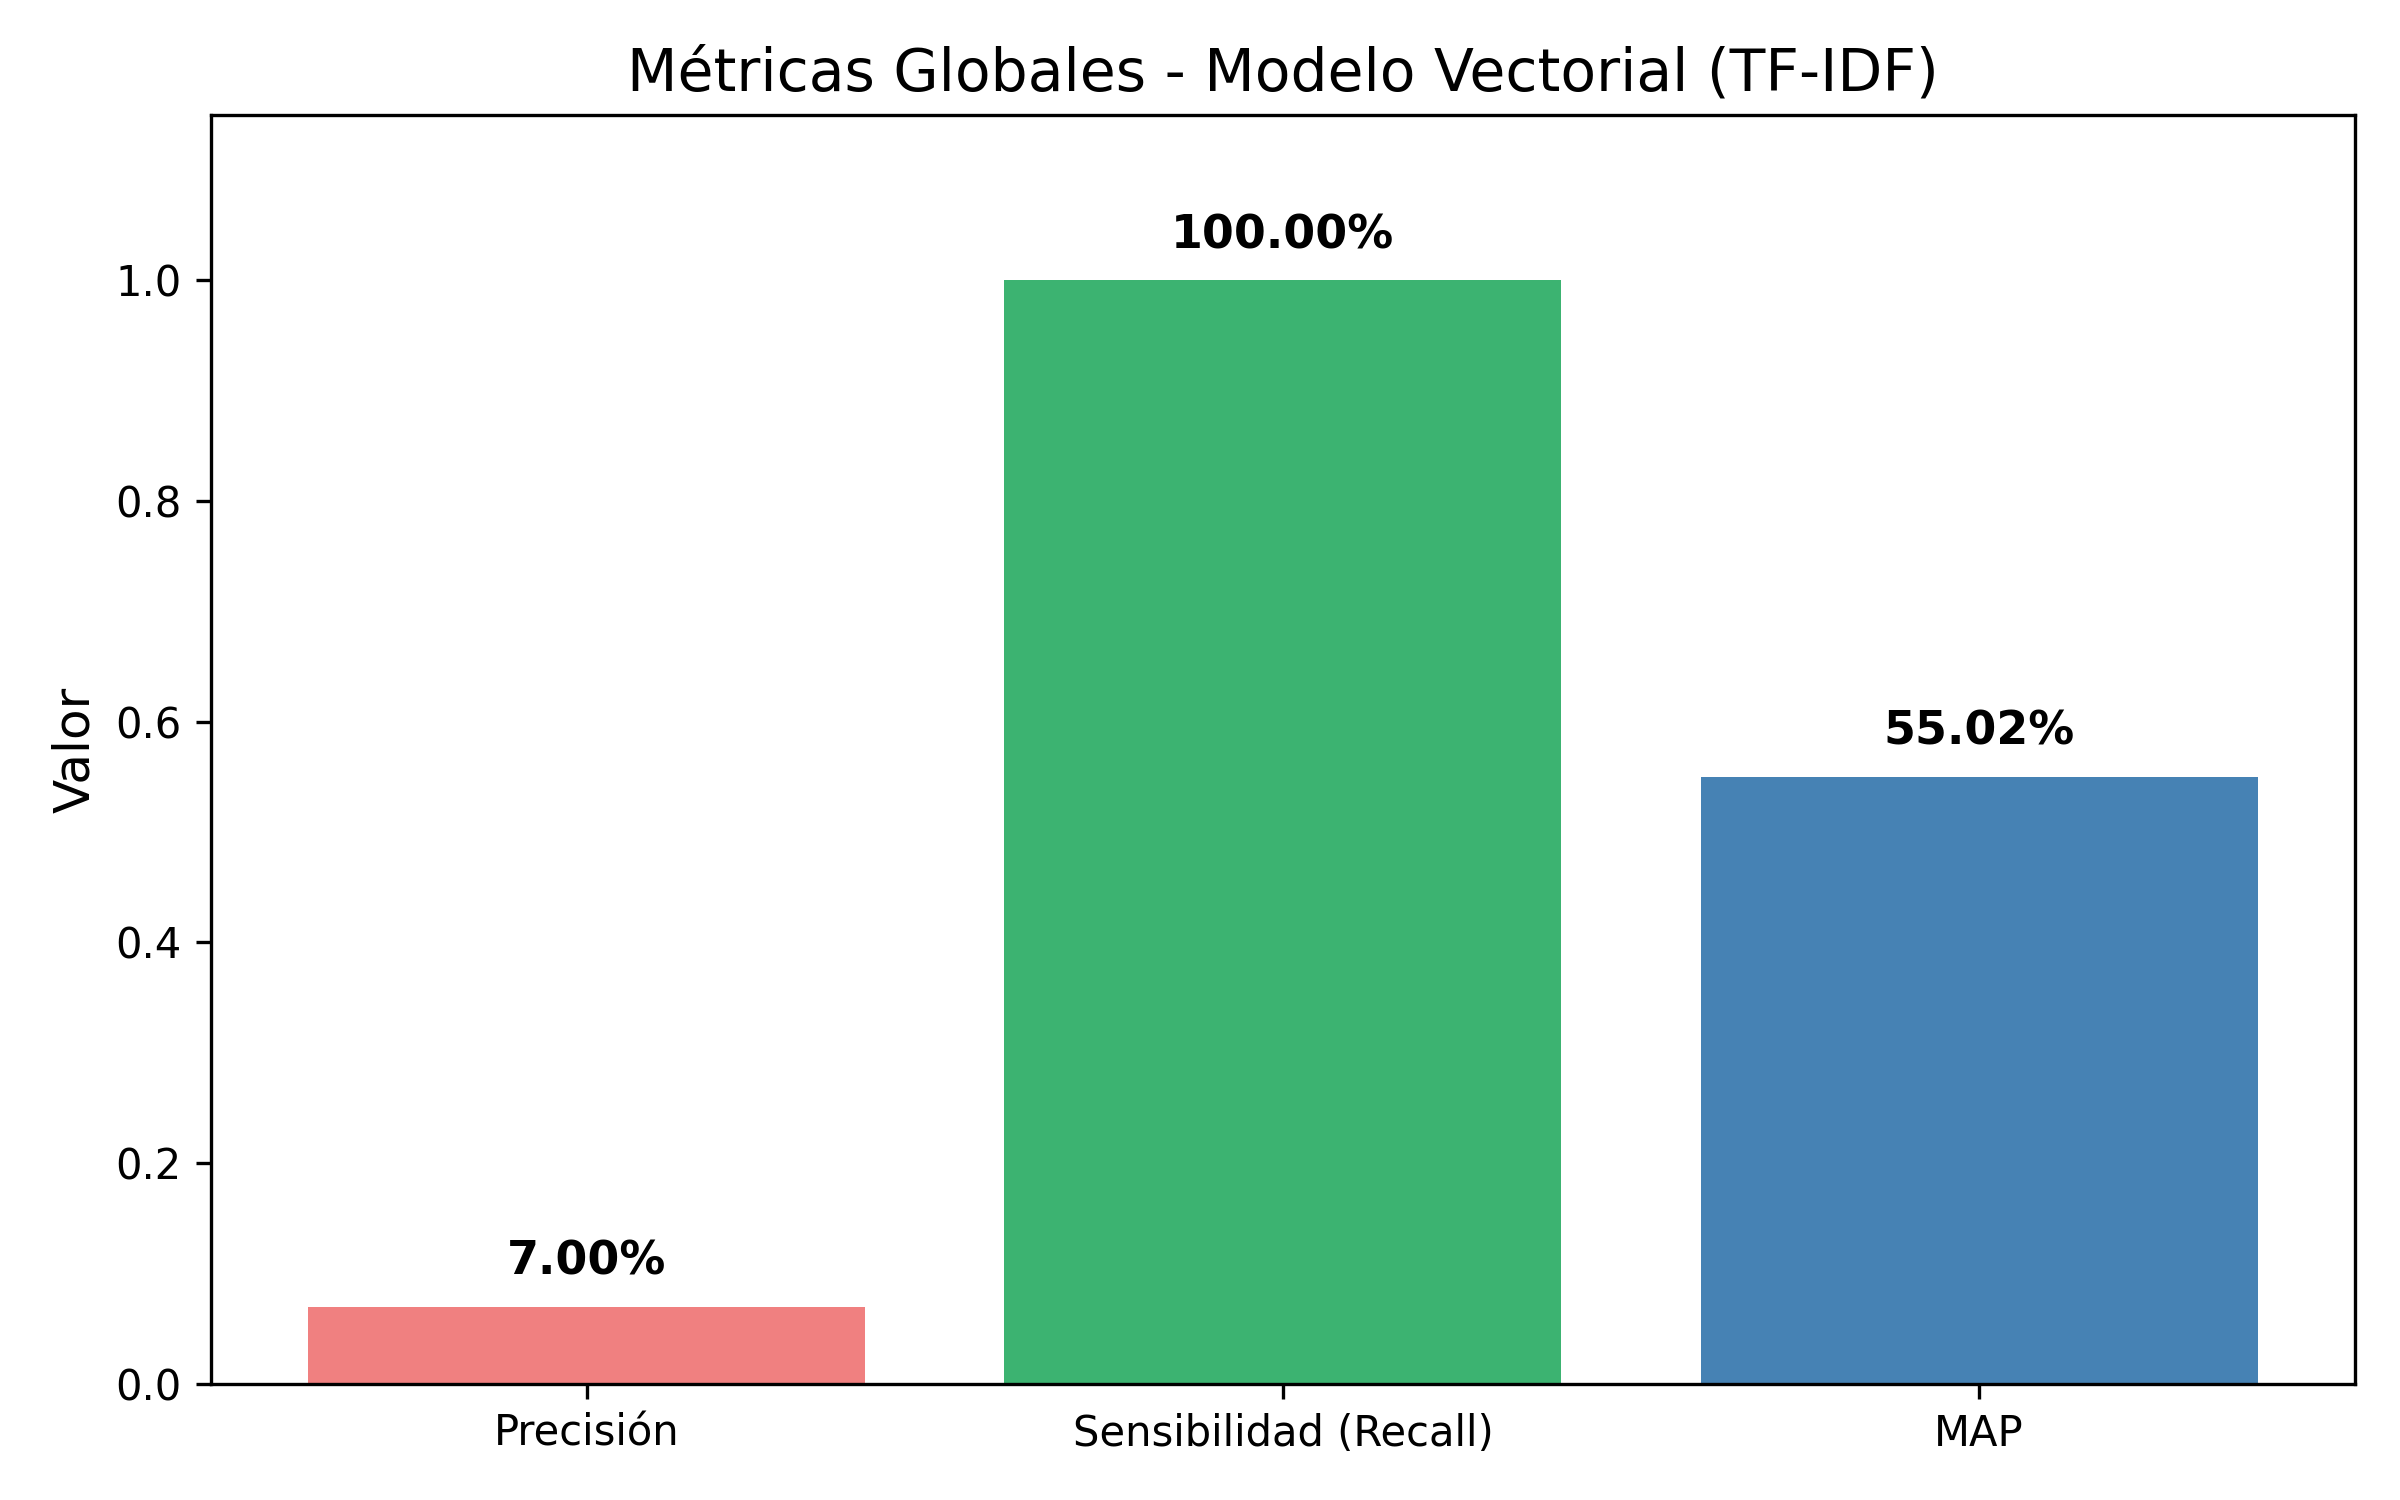
\includegraphics[width=\columnwidth]{metrics_chart}
  \caption{Promedio Global Matemático de las tres grandes métricas evaluadas (Precisión, Sensibilidad, MAP) relativas al Modelo Vectorial TF-IDF empírico en análisis.}
  \label{fig:metrics}
\end{figure}

\subsection{Análisis Crítico de la Sensibilidad y Precisión}

Los resultados evidencian claramente cómo funciona el sistema TF-IDF en la práctica. El rotundo 100\% obtenido en Sensibilidad indica que el motor matemático \emph{nunca} pierde un Pokémon relevante. Dado que el sistema vectorial devuelve cualquier documento que comparta al menos una palabra con la consulta (es decir, donde la similitud del coseno sea mayor a 0), prácticamente se garantiza atrapar a todos los candidatos correctos.

La contrapartida de este enfoque es la inclusión masiva de ruido. Al devolver casi todos los documentos disponibles con una puntuación superior a cero, el número de falsos positivos se dispara, lo que desploma severamente la Precisión pura hasta un marginal 7.00\%. En este aspecto, el modelo Booleano demuestra su indiscutible superioridad a la hora de filtrar el contenido estricto: al requerir condiciones lógicas, la precisión del booleano se mantiene inmensamente alta, aunque a costa de requerir que el usuario sea un experto en el manejo de sintaxis compleja.

A pesar de la baja precisión neta, la viabilidad del sistema vectorial queda completamente refrendada por el **MAP del 55.02\%**. Esta métrica evidencia que el modelo es sumamente eficaz ordenando los resultados. Aunque se incluyan muchos falsos positivos al final de la lista, las operaciones matemáticas logran empujar los documentos verdaderamente relevantes a la codiciada parte alta del ranking, permitiendo que el usuario encuentre lo que busca sin necesidad de conocer la sintaxis booleana.

\subsection{El problema de la Bolsa de Palabras (Bag of Words)}

Uno de los descubrimientos más reveladores demostrados durante esta investigación ha sido constatar de primera mano la principal limitación inherente del modelo vectorial \emph{Bag of Words}: la carencia absoluta de comprensión contextual de las oraciones.

Para ilustrar este punto, al introducir la consulta de rastreo libre \emph{``fast special attacker''}, buscando un Pokémon de corte ofensivo, el sistema determinó sorprendentemente que el documento de mayor similitud de todo el corpus correspondía a Ting-Lu, el famoso tanque defensivo. El error recae unánimemente en que Ting-Lu está clasificado estratégicamente como una ``muralla especial''. Así, el autor del artículo original empleó las palabras \emph{``special''} (62 veces) y \emph{``attacker''} (73 veces) reiteradamente a lo largo del texto precisamente para referirse a que Ting-Lu \emph{bloquea a los atacantes especiales}. 

El motor, siendo ciego a la pragmática y a la sintaxis estructural del idioma, simplemente ponderó la enorme frecuencia bruta de las palabras solicitadas y multiplicó el retorno matemático, creyendo falsamente que el documento encajaba a la perfección con la consulta. Esta inevitable falla algorítmica demuestra la utilidad vital de los modelos Booleanos avanzados, donde el usuario podría añadir un operador de exclusión restrictiva como \texttt{NOT "special wall"} para solventar instantáneamente el falso positivo contextual.

\section{Conclusiones}

Este proyecto multidisciplinar ha logrado materializar eficientemente, estructurar y medir de forma analítica dos potentes paradigmas clásicos de la Recuperación de Información sobre una plataforma funcional puramente estructurada operativamente, evidenciando de modo práctico la teoría estudiada.

El sistema de rastreo estricto Booleano destaca enormemente cuando el usuario que lo emplea domina la terminología y las expresiones lógicas del lenguaje. Su capacidad de filtrado es drástica y precisa, pero su barrera de entrada excluye a quien desconozca cómo formular las expresiones adecuadamente. Por el contrario, el motor de Recuperación Vectorial proporciona una interfaz de búsqueda de texto libre mucho más amigable, obteniendo resultados notables a la hora de ordenar los documentos por relevancia (MAP del 55.02\%) e impidiendo que los documentos relevantes se escapen (Sensibilidad perfecta del 100\%). 

Sin embargo, el sistema Vectorial acusa severamente su incapacidad de entender el contexto de las oraciones, tal y como se comprobó empíricamente con la limitación de la Bolsa de Palabras frente a los contextos defensivos y ofensivos de la literatura de Pokémon. Como paso futuro, se augura la necesaria implementación de entornos basados en Inteligencia Artificial semántica pura (\emph{Word Embeddings}) que entiendan algorítmicamente el peso jerárquico real del texto y los sinónimos directos, erradicando los falsos positivos por contexto cruzado.


\begin{thebibliography}{00}
\bibitem{b1} Smogon University, ``Smogon Strategy Pokedex,'' disponible en: \texttt{https://www.smogon.com/dex/sv/pokemon/}.
\bibitem{b2} C. D. Manning, P. Raghavan y H. Schütze, \emph{Introduction to Information Retrieval}, Cambridge University Press, 2008.
\bibitem{b3} S. Bird, E. Klein y E. Loper, \emph{Natural Language Processing with Python}, O'Reilly Media, 2009.
\bibitem{b4} IIR, Capítulo 1: \emph{Boolean retrieval}, Stanford NLP Group, online.
\bibitem{b5} IIR, Capítulo 6: \emph{Scoring, term weighting, and the vector space model}, Stanford NLP Group, online.
\bibitem{b6} F. Pedregosa et al., ``Scikit-learn: Machine Learning in Python,'' \emph{JMLR}, vol. 12, pp. 2825-2830, 2011.
\bibitem{b7} NLTK Project, ``Natural Language Toolkit,'' disponible en: \texttt{https://www.nltk.org/}.
\bibitem{b8} IIR, Capítulo 8: \emph{Evaluation in information retrieval}, Stanford NLP Group, online.
\end{thebibliography}

\end{document}
